\documentclass[11pt]{amsbook}
\usepackage[turkish]{babel}

\usepackage{../Ceyhun}	% ------------------------
\usepackage{../amsTurkish}
\usepackage{lipsum}

\begin{document}

% =====================================
\begin{proof} \footnote{Proof starts in the previous page. Begin tag should be removed.}
	$$ d - a + y = 2 $$

	$$a \leqslant \frac{2}{3} a + \frac{1}{3} a - 2$$

	$$0 \leqslant -2$$

	elde ederiz. Bu çelişki, ancak $y_3 = y_4 = y_5 = 0$
	koşulunu kaldırarak giderilebilir.
\end{proof}

% =====================================
\begin{definition}
	Belli bir i ve j için,
	$y=y_i$ ve $d=d_j$
	koşulunu sağlayan çokyüzlülere
	\hDefined{düzgün çokyüzlü} denir.
\end{definition}

Düzgün çokyüzlülere verilebilecek beş örneğin
düzlemsel çizimleri \reffig{fig:DuzgunCokyuzluler} \footnote{The figure continues in the next page. 
									End, label and caption tags should be adjusted accordingly.}
de gösterilmiştir.

% =====================================
\begin{figure}[htb]
	\centering
	\subfigure[]{
 		\label{fig:DuzgunCokyuzlulerA}
 		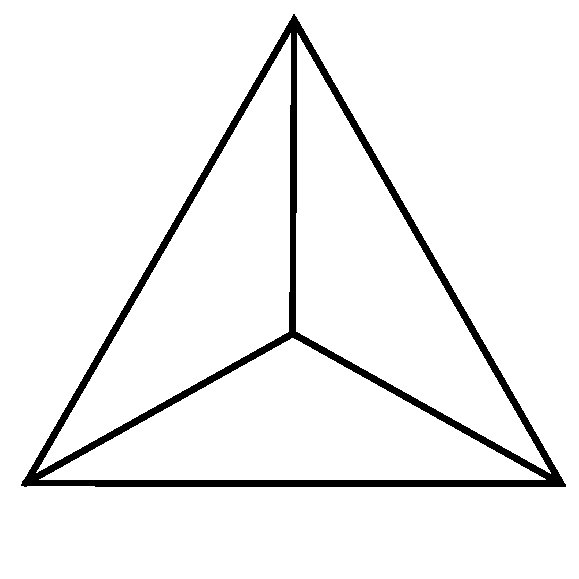
\includegraphics[width=0.25\linewidth]{images/ceyhun-182-fig01a}
 	}
	\hspace*{0.15\linewidth} % separation between the subfigures
	\subfigure[]{
 		\label{fig:DuzgunCokyuzlulerA}
 		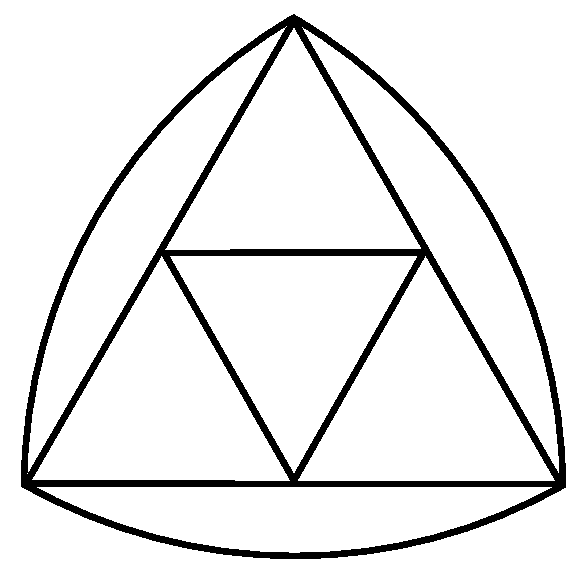
\includegraphics[width=0.25\linewidth]{images/ceyhun-182-fig01b}
	}
	\label{fig:DuzgunCokyuzluler}
\end{figure}

% =====================================

\end{document}